\section{Fits}
\label{s:fits}

Data presented in fig. 4 from \cite{PhysRevLett.105.167202}
was fit
\footnote{
  Fits done using the
  \href{https://github.com/razor-x/scipy-data_fitting}{scipy-data\_fitting} Python package.
  The source code used to generate these fits is hosted at
  \href{https://github.com/razor-x/spin-lifetime-analysis}{github.com/razor-x/spin-lifetime-analysis}.
  The source code used to generate the figures is hosted at
  \href{https://github.com/razor-x/aps-spin-lifetime-plots}{github.com/razor-x/aps-spin-lifetime-plots}.
  The commits pointing to a snapshot of the code used for this paper
  are tagged as releases with the name \texttt{PhysRevLett}.
}
\cite{Hunter:2007}
to the model presented here.
We assume similar contacts, $R_C = R_C^0 = R_C^L$.
The resistance of the ferromagnet \ce{Co} is computed as
$R_F = ρ_F λ_F / A_J$,
where $A_J$ is the junction area estimated at $A_J = W d$,
with $d$ between \SIrange[range-phrase={ and }]{0.5}{50}{\nano \meter}
\cite{PhysRevLett.105.167202}.
Hanle fits were done using a simple least squares algorithm
with nonnegative parameters $τ$, $D$, $R_C$, and $P$.
The polarization $P$ was constrained between zero and one.

\begin{figure}[b]
  \caption{
    Data in fig. 4 from \cite{PhysRevLett.105.167202}
    fit to \cref{eq:nonlocal_resistance.difference}
    with the following values: \plotDifferenceInfo.
    The contact type (tunneling or transparent)
    and the contact separation $L$ varies.
  }
  \label{fig:nonlocal_resistance.difference}
  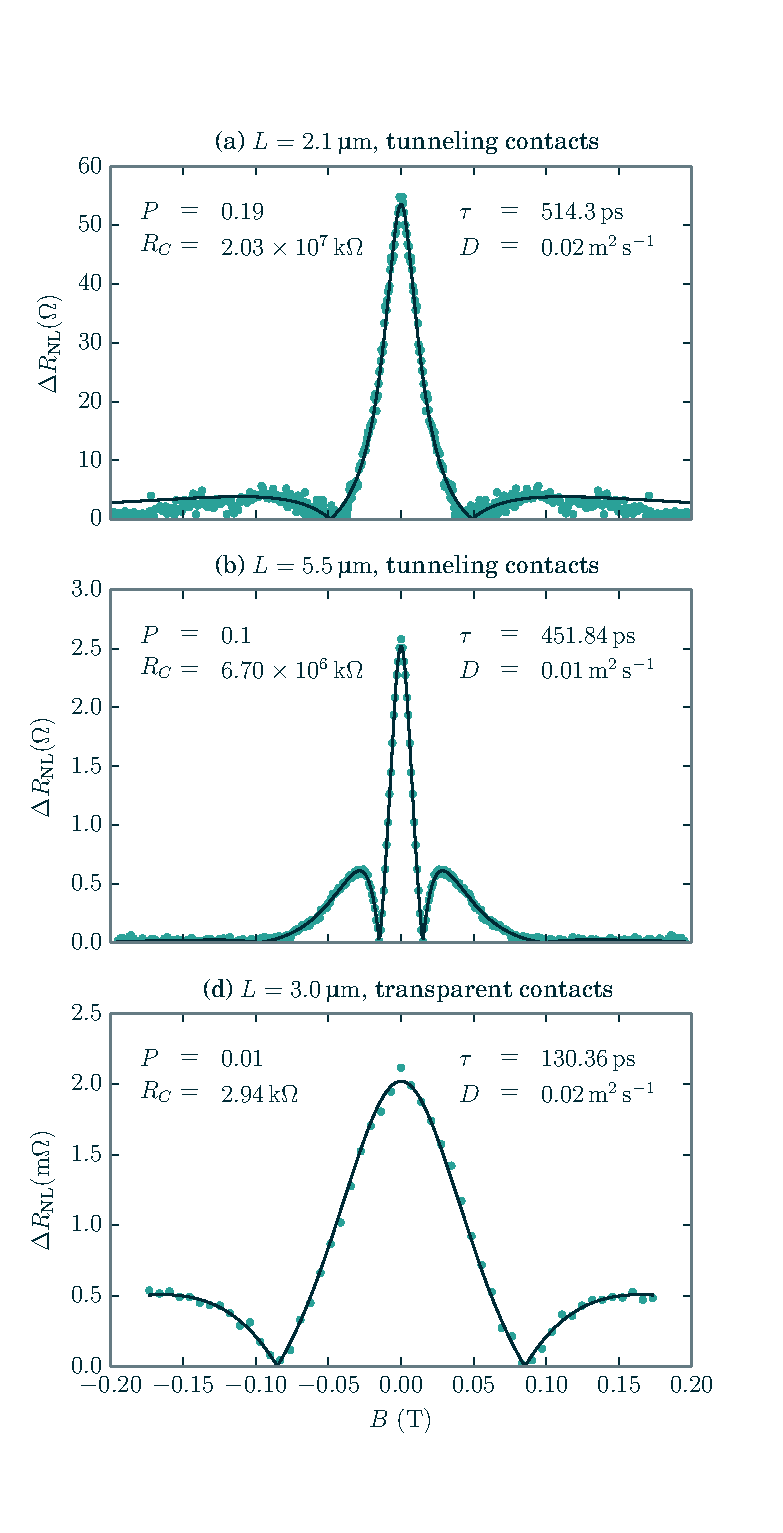
\includegraphics[width=\columnwidth]{figures/plot_difference}
\end{figure}

\Cref{fig:nonlocal_resistance.difference} shows fits of
$Δ \rNL$ given by \cref{eq:nonlocal_resistance.difference}
for devices with tunneling and transparent contacts.
Fits (a) and (b) with tunneling contacts give large
$R_C ∼ \SI{e7}{\kilo \ohm}$ and lifetimes equivalent to fitting with $R_C → ∞$,
while (d) with transparent contacts gives a reduced $R_C ∼ \SI{3}{\kilo \ohm}$
and a lifetime increased by at most a factor of two
(compare to \SI{78}{\pico \second} for $R_C → ∞$).
For tunneling contacts, the polarization $P$ is \SIrange{25}{60}{\percent}
smaller than the lower bound given in \cite{PhysRevLett.105.167202},
while for transparent contacts, $P$ is reduced by an order of magnitude.

\begin{figure}
  \caption{
    Data in fig. 4 (c) from \cite{PhysRevLett.105.167202}
    fit to \cref{eq:nonlocal_resistance}
    with the following values: \plotParallelInfo.
    The contact is pinhole type.
  }
  \label{fig:nonlocal_resistance.pinhole}
  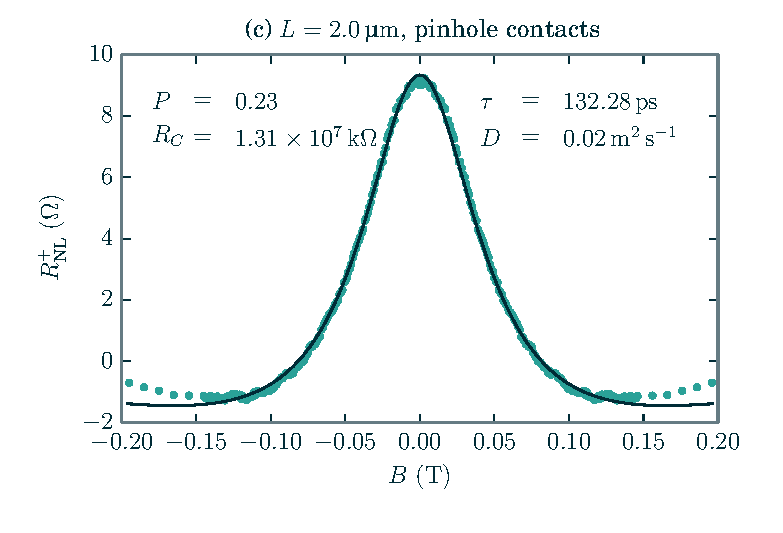
\includegraphics[width=\columnwidth]{figures/plot_parallel}
\end{figure}

\Cref{fig:nonlocal_resistance.pinhole} shows a fit of
$\rNL^+$ given by \cref{eq:nonlocal_resistance}
with $p_1 p_2 → P^2$ for a device with pinhole contacts
\footnote{
  Parallel and antiparallel data for this device was only available
  at dissimilar field values, thus $Δ \rNL$ could not be fit.
}.
The lifetime is equivalent to fitting with $R_C → ∞$.

Note that we have used $R_C$ as a fitting parameter.
In most devices, this is quantity can be experimentally determined
helping further constrain the fitting algorithm.
As we will discuss further in the next section, a fact that becomes apparent
from our analytic result is that the relevant scale is $λ / r$.
Once $r$ becomes larger than $λ$,
all of the corrections to the $R_C → ∞$ limit Hanle curves become very small.
In other words, once $r ≫ λ$,
the fit is insensitive to the actual value of the contact resistance.
The fact that we quote resistance of order \SI{e7}{\kilo \ohm} in fits (a), (b), and (c)
in \cref{fig:nonlocal_resistance.difference,fig:nonlocal_resistance.pinhole}
results from the built-in accuracy we demand of the fitting algorithm.
A good fit can be obtained for any $r$ as long as it is larger than $λ$.
